\newpage
\chapter{Proposed Methodology}

\section{System Architecture}
Mitsuketa follows a three-tier architecture:
\begin{enumerate}
  \item \textbf{Presentation Layer:} A React/Vite Single-Page Application (SPA) communicating with the backend via HTTP fetch calls.
  \item \textbf{Business Logic Layer:} A FastAPI ASGI server running Python fingerprinting and matching algorithms.
  \item \textbf{Data Layer:} A highly scalable \textbf{PostgreSQL 18} database managing users, roles, and media fingerprints with complex query optimization.
\end{enumerate}

The modular design ensures that each layer can be independently scaled. The PostgreSQL database structure combined with BK-Tree indexing allows production-scale deployment without modifying the core fingerprinting logic.

\begin{figure}[h!]
  \centering
  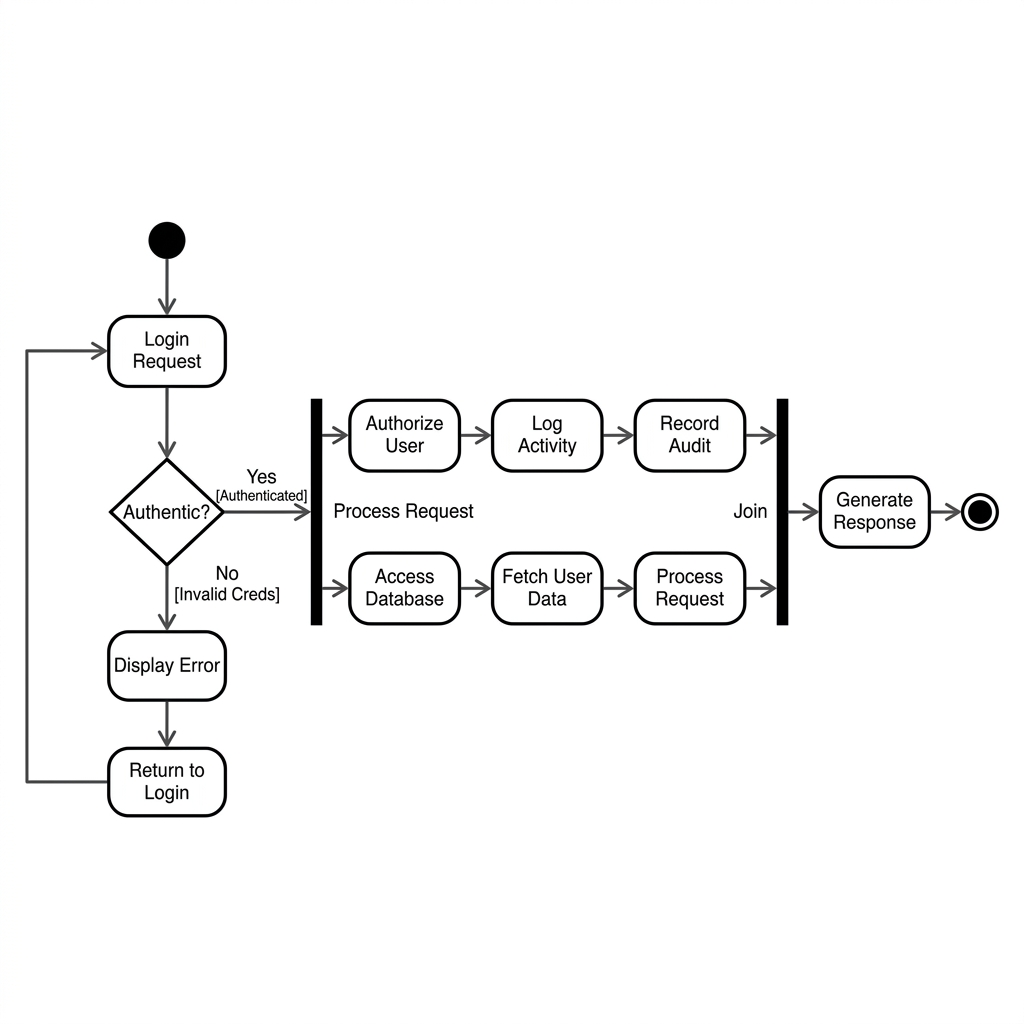
\includegraphics[width=0.97\textwidth]{WorkFlow}
  \caption{Multimedia Content Matching Workflow: End-to-End Identification Pipeline}\label{fig:workflow}
\end{figure}

\section{Mathematical Modeling}

\subsection{Audio Fingerprinting: Short-Time Fourier Transform (STFT)}
The first step in audio fingerprinting is to transform the raw time-domain audio signal $x(t)$ into a time-frequency spectrogram $S(t, f)$ using the Short-Time Fourier Transform:
\begin{equation}
  S(t, f) = \sum_{n=-\infty}^{\infty} x[n] \cdot w[n - t] \cdot e^{-j2\pi f n}
\end{equation}
where $w[n]$ is a window function (Hann window) of duration $T_w$. The magnitude spectrogram $|S(t, f)|^2$ is used to identify high-energy ``peak'' points in the time-frequency plane.

\subsection{Constellation Map Hashing}
Each peak $p_i = (t_i, f_i)$ is paired with surrounding ``target'' peaks $p_j = (t_j, f_j)$ within a fan-out zone to generate a hash:
\begin{equation}
  H_{ij} = \text{SHA1}\left( f_i \mathbin\| f_j \mathbin\| (t_j - t_i) \right)_{[0:20]}
\end{equation}
where $\|$ denotes concatenation. The 20-character truncated SHA-1 string forms the fingerprint hash. Each hash is stored alongside the anchor time offset $t_i$ (the absolute time in the original media).

\begin{figure}[h!]
  \centering
  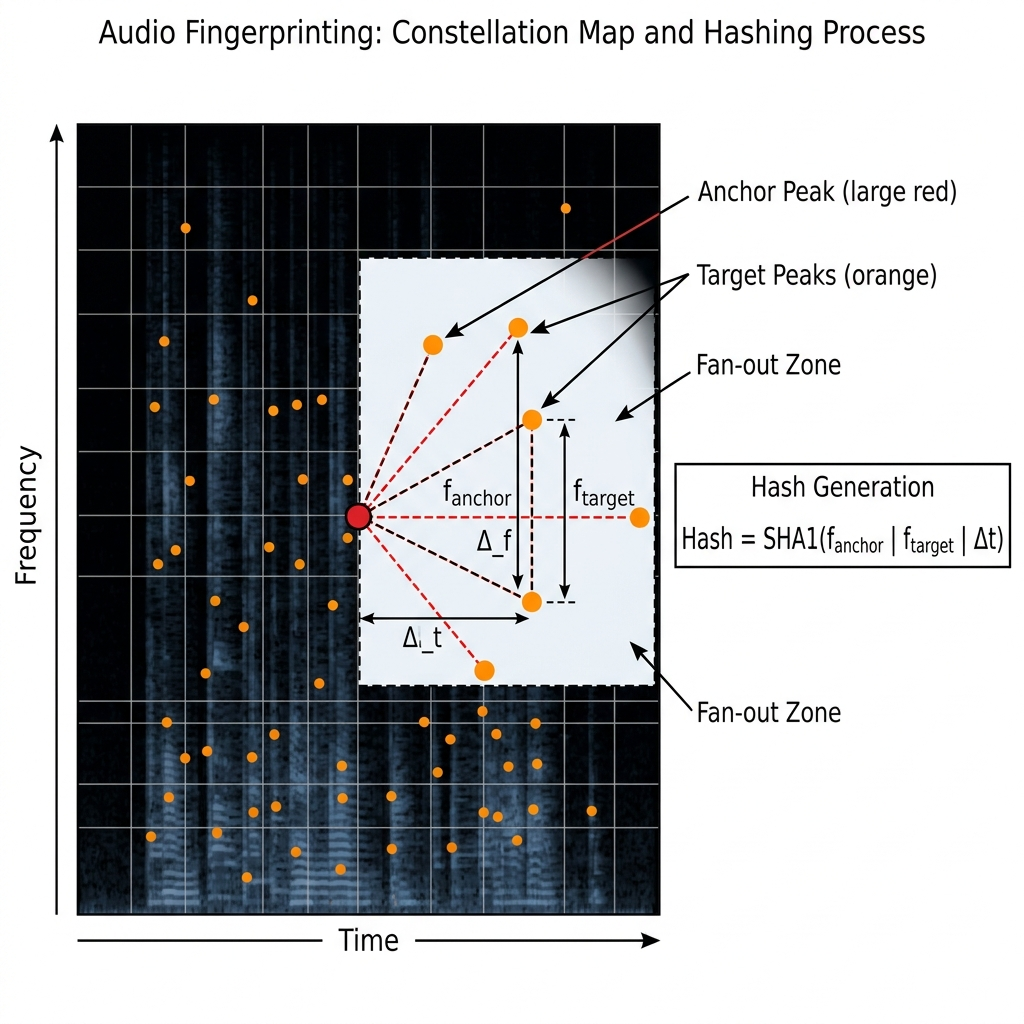
\includegraphics[width=0.90\textwidth]{audio_constellation_map}
  \caption{Constellation Map: Anchor-Target Peak Pairing and Hash Generation}\label{fig:constellation}
\end{figure}

\subsection{Temporal Alignment for Matching}
During identification, query hashes are compared against database hashes. A successful match requires:
\begin{equation}
  \Delta t = T_{\text{db}} - T_{\text{query}} = \text{constant}
\end{equation}
across many matching hashes. The number of hashes sharing the same offset $\Delta t$ defines the alignment strength, which directly drives the audio confidence $C_{\text{audio}}$.

\subsection{Perceptual Hashing (pHash) for Video}
For a keyframe image $I$, the pHash is computed as:
\begin{enumerate}
  \item Resize $I$ to $32 \times 32$ pixels and convert to grayscale.
  \item Apply a 2D Discrete Cosine Transform (DCT):
  \begin{equation}
    D[u,v] = \sum_{x=0}^{N-1}\sum_{y=0}^{N-1} I[x,y] \cos\!\left[\frac{\pi(2x+1)u}{2N}\right]\cos\!\left[\frac{\pi(2y+1)v}{2N}\right]
  \end{equation}
  \item Extract the top-left $8 \times 8$ block of $D[u,v]$ (low-frequency coefficients).
  \item Compute the mean $\mu$ of the 64 coefficients.
  \item Binarize: $h[i] = 1$ if $D_i > \mu$, else $h[i] = 0$.
  \item Encode the 64-bit result as a 16-character hexadecimal string.
\end{enumerate}

\begin{figure}[h!]
  \centering
  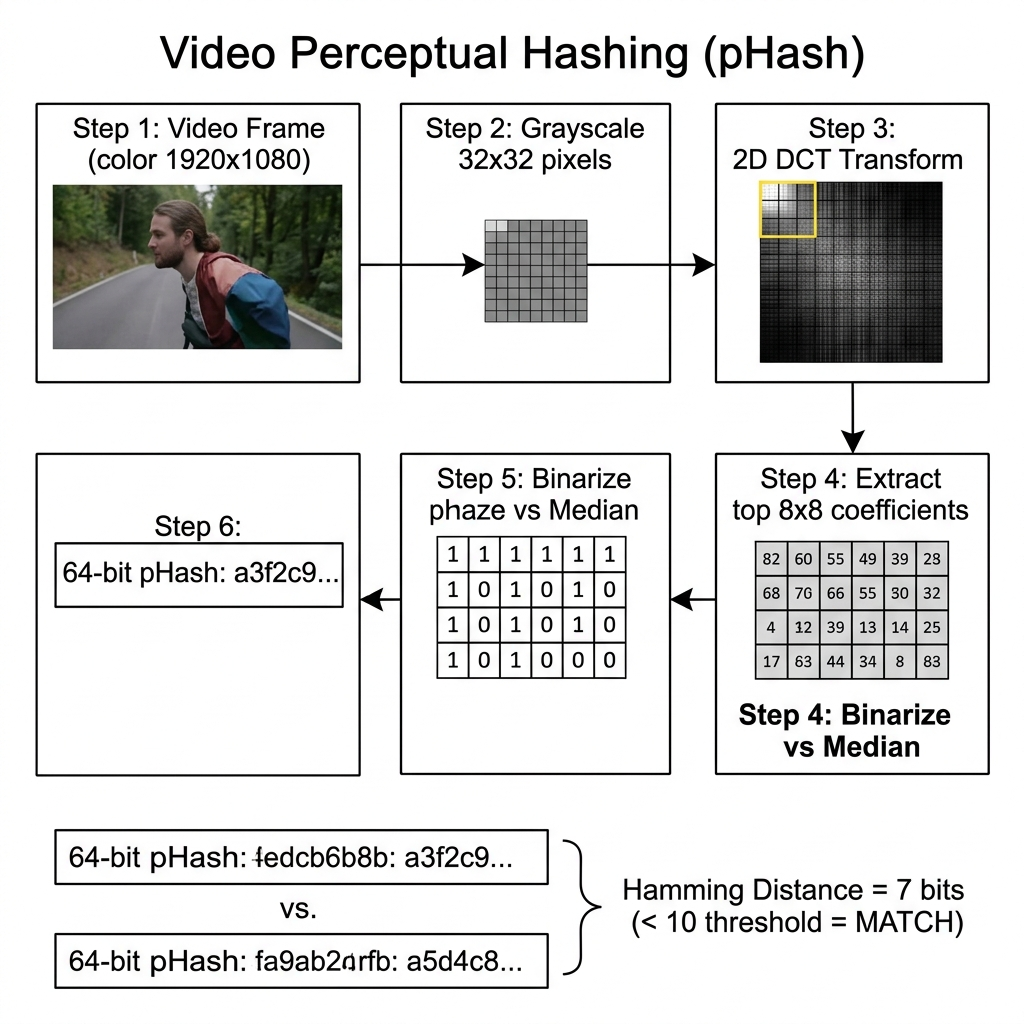
\includegraphics[width=0.92\textwidth]{phash_pipeline}
  \caption{Video Perceptual Hashing (pHash) Pipeline: From Frame to 64-bit Hash}\label{fig:phash}
\end{figure}

The \textbf{Hamming distance} between two pHashes $h_A$ and $h_B$ is the number of bit positions at which the two values differ:
\begin{equation}
  d_H(h_A, h_B) = \text{popcount}(h_A \oplus h_B)
\end{equation}
A Hamming distance of $d_H < 10$ (out of 64 bits) is used as the threshold for a visual match.

\subsection{BK-Tree for Logarithmic Video Search}
The BK-Tree (Burkhard-Keller Tree) is constructed using the Hamming distance metric. For a database of $N$ video hashes:
\begin{itemize}
  \item \textbf{Construction:} $O(N \log N)$ average time.
  \item \textbf{Query:} $O(\log N)$ average time for finding all hashes within distance $d \leq \tau$.
\end{itemize}
This provides a significant performance improvement over the $O(N)$ brute-force linear scan, especially as the media library grows to thousands of titles.

\begin{figure}[h!]
  \centering
  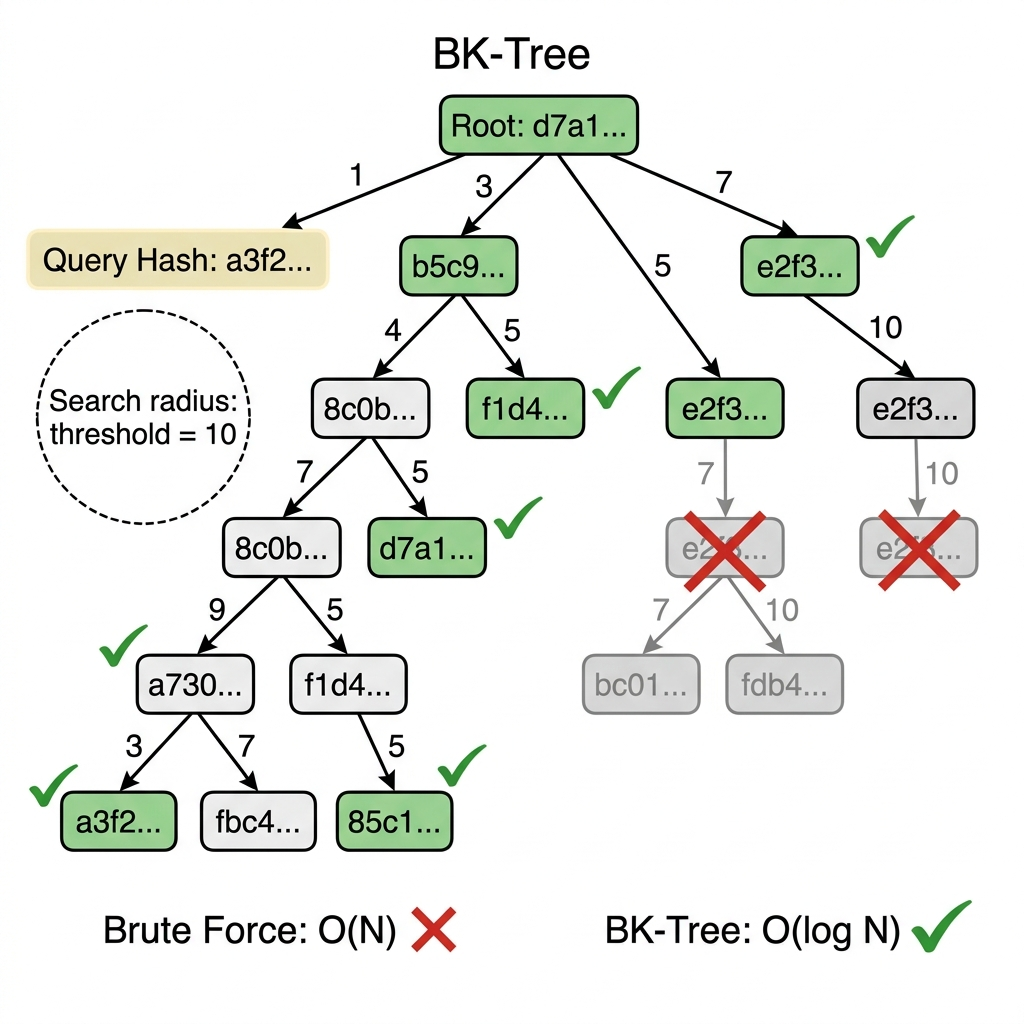
\includegraphics[width=0.88\textwidth]{bktree_structure}
  \caption{BK-Tree Structure for Logarithmic Hamming Distance Search}\label{fig:bktree}
\end{figure}

\section{Objective Function}
The overall system objective is to maximize identification accuracy $A$ while minimizing query latency $L$:
\begin{equation}
  \underset{\theta}{\text{maximize}} \quad A(\theta) = \frac{\text{Correctly Identified Queries}}{\text{Total Queries}}
\end{equation}
\begin{equation}
  \text{subject to} \quad L \leq L_{\max}
\end{equation}
where $\theta$ represents the system parameters (e.g., fan-out zone size, BK-Tree distance threshold $\tau$, audio confidence threshold $\alpha$) and $L_{\max} = 2$ seconds is the acceptable maximum query latency.

\section{Approach}
The development follows an iterative build-test-refine cycle:
\begin{enumerate}
  \item Implement and validate the audio fingerprinting pipeline independently using known audio clips.
  \item Implement and validate the video fingerprinting pipeline independently.
  \item Integrate both pipelines with the FastAPI backend and SQLite storage layer.
  \item Build the React frontend and connect it to the API.
  \item Run structured test cases (noisy audio, resized video, combined) and tune the confidence threshold parameters.
\end{enumerate}

\vspace{10mm}
\hrule